\documentclass[12pt,a4paper]{ctexart}
\usepackage{geometry}
\usepackage{amsmath}
\usepackage{amssymb}
\usepackage{graphicx}
\usepackage{enumerate}
\usepackage{enumitem}
\usepackage{xcolor}
\usepackage{fancyhdr}
\usepackage{titlesec}

% 页面设置
\geometry{left=2.5cm,right=2.5cm,top=2.5cm,bottom=2.5cm}

% 页眉页脚设置
\pagestyle{plain}

% 标题格式设置
\titleformat{\section}{\Large\bfseries}{\chinese{section}、}{0em}{}
\titleformat{\subsection}{\large\bfseries}{\arabic{subsection}、}{0em}{}

% 文档开始
\begin{document}

% 标题部分
\begin{center}
    \LARGE\textbf{《射频电路与系统》回忆卷}
\end{center}

\vspace{0.5cm}

% 判断题
\section{判断题（1pt$\times$10）}

\begin{enumerate}[label=\arabic*、,leftmargin=2em]
    \item 模拟噪声系统的噪声系数大于1 \hfill （\quad）
    
    \item 串联谐振回路中电感与电容的电压同相 \hfill （\quad）
    
    \item 回路的矩形系数反应了回路的带宽 \hfill （\quad）
    
    \item 晶体振荡器提高频率范围的方法是在后串联电感 \hfill （\quad）
    
    \item 锁相环的基本功能是使输出频率等于输入频率 \hfill （\quad）
    
    \item C类放大器中添加扼流圈是为了在相同功率下降低电源电压 \hfill （\quad）
    
    \item 增益压缩点是信号自身的二阶失真 \hfill （\quad）
\end{enumerate}

\vspace{1cm}

% 填空题
\section{填空题（30pt，一空一分）}

\begin{enumerate}[label=\arabic*、,leftmargin=2em]
    \item LNA要尽可能的大，是为了放大\underline{\hspace{3cm}}，改善\underline{\hspace{3cm}}，但LNA的增益不宜太高，太高变频器会\underline{\hspace{3cm}}，BPF1放在LNA后可以降低系统\underline{\hspace{3cm}}，BPF1放在LNA前可以减少\underline{\hspace{3cm}}
    
    \vspace{0.5cm}
    
    \item 混频器工作在\underline{\hspace{3cm}}（选项：非线性、时变、线性时变）状态，这种状态中信号大小是\underline{\hspace{3cm}}（选项：两大，一大一小，两小），其中时变跨到由\underline{\hspace{3cm}}信号控制，输出信号与\underline{\hspace{3cm}}信号呈线性
    
    \vspace{0.5cm}
    
    \item 反馈型振荡器自起振的过程中\underline{\hspace{3cm}}（选项：$AF>1$，$AF=1$，$AF<1$），平衡时\underline{\hspace{3cm}}（选项：$AF>1$，$AF=1$，$AF<1$），晶体管从自起振到平衡利用了其三个效应\underline{\hspace{3cm}}、\underline{\hspace{3cm}}、\underline{\hspace{3cm}}
    
    \vspace{0.5cm}
    
    \item C类功率放大器的导通角\underline{\hspace{3cm}}，其效率高的核心原因是\underline{\hspace{3cm}}
    
    \vspace{0.5cm}
    
    \item 影响振荡器频率稳定度最大的是\underline{\hspace{3cm}}（选项：白噪声、相位噪声、幅度噪声），上混频是将信号转移到\underline{\hspace{3cm}}（选项：射频带，中频带，基带），下混频是将信号转移到\underline{\hspace{3cm}}（选项：射频带，中频带，基带），如果有强干扰源还会产生\underline{\hspace{3cm}}混频
\end{enumerate}

\vspace{1cm}

% 简答题
\section{简答题（5pt$\times$6）}

\begin{enumerate}[label=\arabic*、,leftmargin=2em]
    \item 源和负载有哪几种匹配，分别起什么作用，一般系统是什么匹配
    
    \item 给出IP3,IIP3,OIP3的定义并画出曲线图
    
    \item LNA相较于低频放大器的区别是什么，除了放大，设计LNA时还需要考虑什么问题
    
    \item 普通三点式振荡器（考毕兹振荡器）有什么缺点？如何改进？改进后有什么优点和缺点？
    
    \item 给出单环锁相环分频器的原理框图，相较于普通锁相环，有什么性能区别
    
    \item 相较于三极管混频器，吉尔伯特混频器有什么优点，理想乘法用的是什么乘法，为什么一般不常用
\end{enumerate}

\newpage

% 计算题
\section{计算题（10pt$\times$3）}

\begin{enumerate}[label=\arabic*、,leftmargin=2em]
    \item \textbf{（共10分）}
    
    \begin{center}
        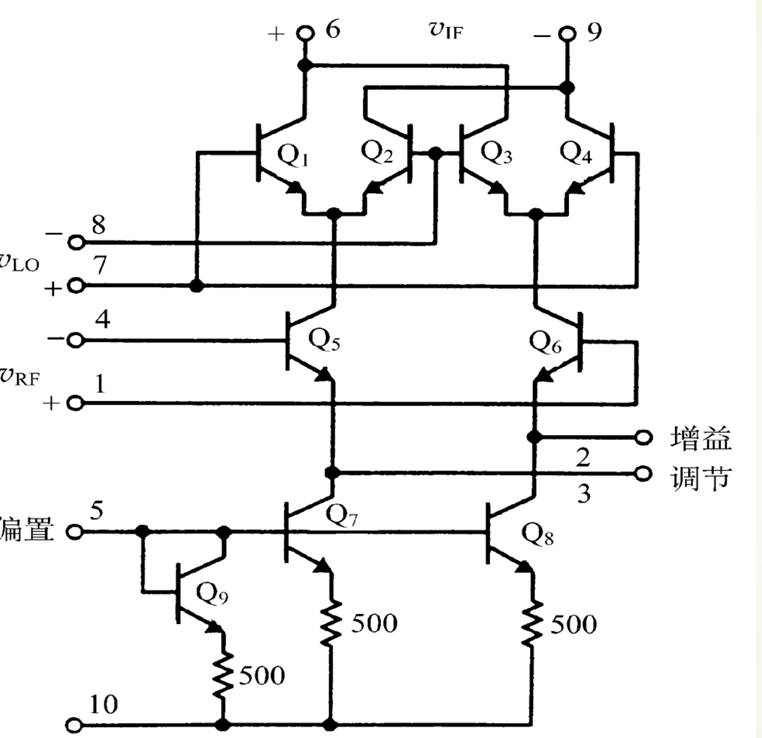
\includegraphics[width=0.8\textwidth]{p1.png}
    \end{center}
    
    \vspace{0.5cm}
    
    \begin{enumerate}[label=（\arabic*）,leftmargin=3em]
        \item 这是什么电路，射频口，本振口，输出口怎么接（4pt）
        
        \item 画出移相网络功能，并说明移相网络的两个功能（4pt）
        
        \item 如何连接移相网络与此电路（2pt）
    \end{enumerate}
    
    \item \textbf{（共10分）}
    
    给出电路，遮住LNA1, LNA2与一些滤波器（还把末端正交鉴频移相网络删了，可能怕你抄到第一题），给出881MHz与最末端的455kHz，将II混频器改为50MHz
    
    \begin{center}
        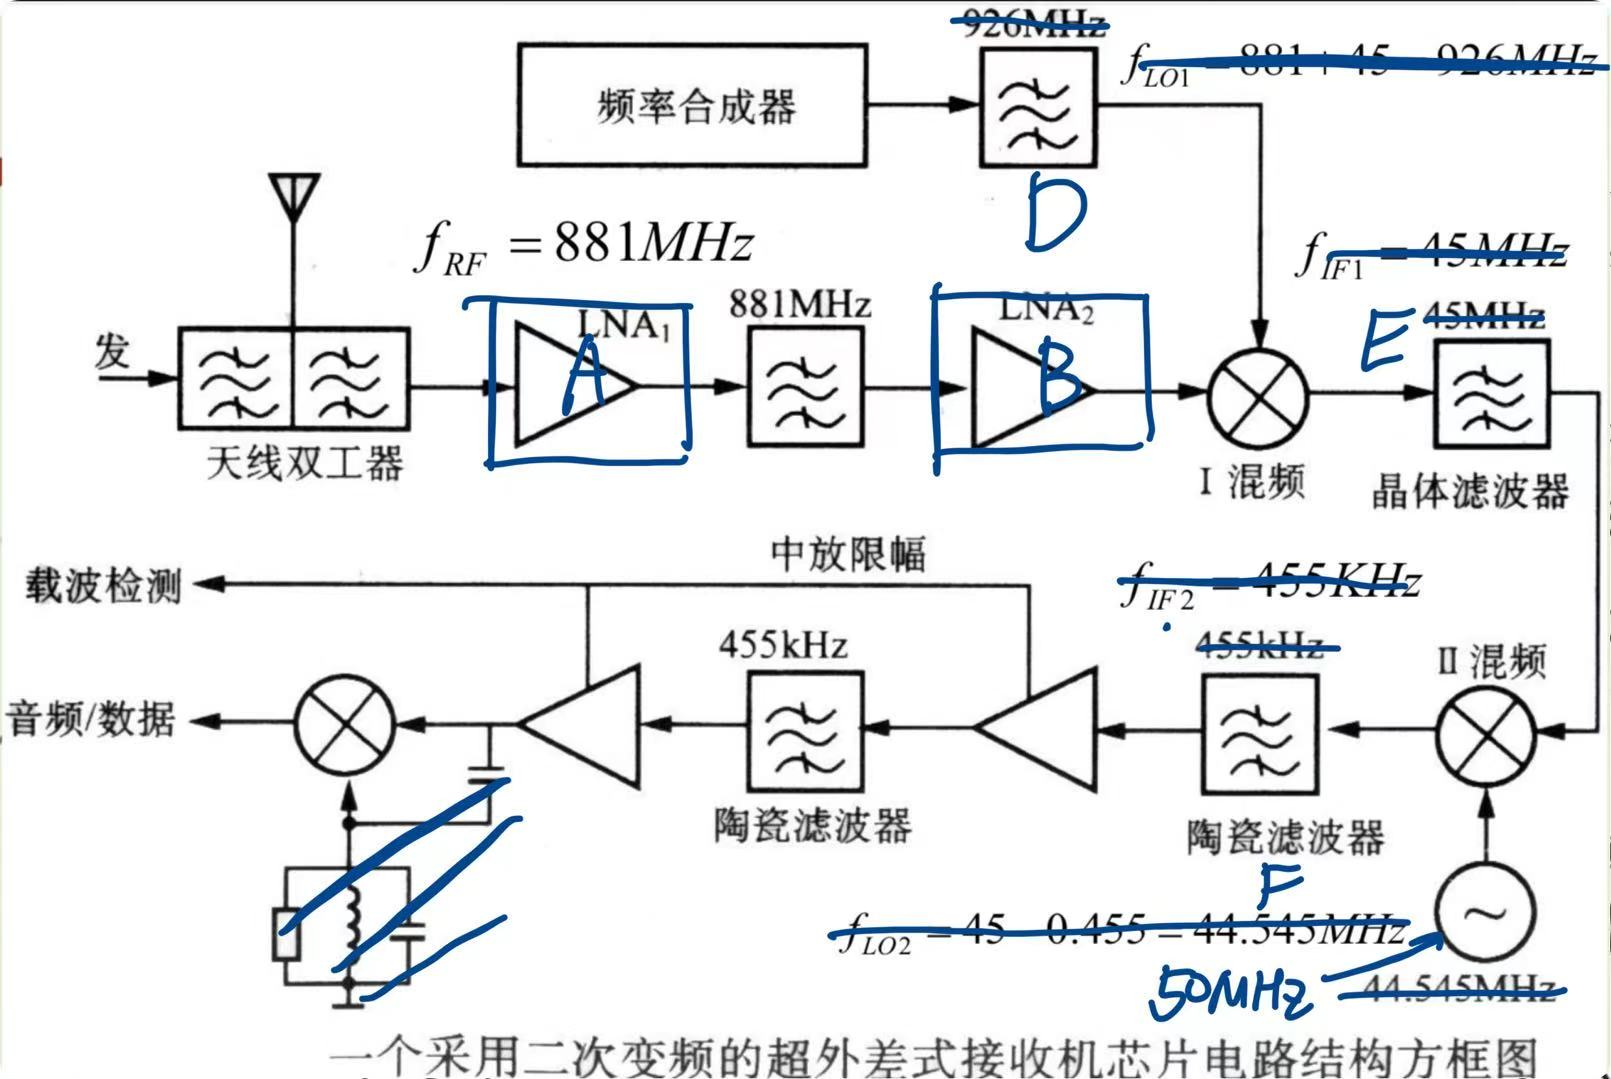
\includegraphics[width=0.8\textwidth]{p2.jpg}
    \end{center}
    
    \vspace{0.5cm}
    
    \begin{enumerate}[label=（\arabic*）,leftmargin=3em]
        \item 这是什么电路？从先到后简述一下信号的流动
        
        \item D, E, F的频率分别是多少，列出所有可能性
    \end{enumerate}
    
    \item \textbf{（共10分）}
    
    习题8-1，将鉴相灵敏度改为3V/rad
    
    \begin{enumerate}[label=（\arabic*）,leftmargin=3em]
        \item 同步带大小，环路能否锁定
        
        \item 稳态相位误差是多少，控制电压多大
    \end{enumerate}
\end{enumerate}

\end{document}
